\chapter{Konzeption der Anwendung}
\thispagestyle{fancy}
\label{chap:concept}

Zu beginn sind der genaue Rahmen und der Ablauf der Anwendung zu definieren. Hierfür muss zunächst der Stand aus dem Praxisprojekt evaluiert werden, um festzustellen, an welchen Stellen weitere Konzeptionsarbeit geleistet werden muss um eine konkrete Umsetzung der Konzepte zu ermöglichen.\\
Das folgende Kapitel beschäftigt sich mit der Spezifizierung des generellen Ablaufes der Anwendung und geht darauf folgend auf die einzelnen Abschnitte ein.

\section{Generelle Struktur der Anwendung}
Innerhalb des Praxisprojektes wurden verschiedene Themengebiete behandelt, die zunächst auf eine Umsetzbarkeit hin validiert werden müssen. Die im Praxisprojekt definierten Themengebiete \cite{PoplawskiPP} sind:

\begin{itemize}
  \item Typographie
  \item Layout \& Struktur
  \item Whitespace
  \item Farben
  \item Bilder
  \item Interaktive Elemente
\end{itemize}

Der Bereich \textit{Whitespace} konnte für eine Umsetzung schnell ausgeschlossen werden, da obgleich seiner Wichtigkeit für eine gute Gestaltung währen des Praxisprojektes keine Konzepte gefunden werden konnten, auf deren Basis eine Umsetzung möglich wäre.\\
Vor der Zielsetzung, innerhalb der Abschlussarbeit eine Marktfähige (und damit in ihren Features vollständige) Anwendung zu erstellen und der gegebenen Zeit von 9 Wochen für deren Umsetzung, muss die Liste der zu behandelnden Gebiete noch weiter eingeschränkt werden.\\
Die Bereiche \textit{Bilder} und \textit{Interaktive Elemente} zeigen im Vergleich die niedrigste Relevanz für eine grundlegende Gestaltung auf. Der Bereich \textit{Bilder} ist ein eher technischer, der sich auf die korrekte Handhabung von Bildern fokussiert. Der Bereich \textit{Interaktive Elemente} ist zwar auch für die Grundlagen der Gestaltung von großer Bedeutung, jedoch ist dieser nur für zwei der drei definierten Zielmedien der Nutzer (vgl. Kapitel \ref{chap:einstieg}) von Bedeutung (Interaktive Elemente kommen in Textdokumenten nicht vor). Hieraus ergibt sich als Liste von Themen für die Umsatzung innerhalb der Abschlussarbeit:

\begin{itemize}
  \item Typographie
  \item Layout \& Struktur
  \item Farben
\end{itemize}

Außerdem sollten für die Anwendung jeweils ein nutzerfreundlicher Einstieg und Ausstieg gefunden werden. Diese wurden im Praxisprojekt nicht explizit ausgearbeitet und fallen somit auch Konzeptionell in den Bereich der Abschlussarbeit und werden später in diesem Kapitel behandelt.
Die finale Struktur der Anwendung für den Rahmen dieser Arbeit sieht also wie folgt aus (der Bereich \textit{Layout \& Struktur} wurde dabei in \textit{Layout \& Grids} umbenannt):

\begin{itemize}
  \item Einstieg
  \item Typographie
  \item Layout \& Grids
  \item Farben
  \item Ausstieg
\end{itemize}

\section{Einstieg in die Anwendung}
\label{chap:einstieg}
Bereits im Praxisprojekt wurde festgestellt, dass es sinnvoll ist, das Zielmedium des Nutzers zu kennen:

\begin{quote}
  Da sich dieses Tool nicht über die plattformspezifischen Richtlinien hinwegsetzen soll, sollte
von Anfang an die Plattform, für die der Nutzer gestaltet, bekannt sein. Die Inhalte des Tools
sollten sich dementsprechend anpassen. \cite{PoplawskiPP}
\end{quote}

Für die Zielgruppe der Studenten wurden hier drei mögliche Zielmedien definiert: Native App, Website und Textdokument. Diese Zielmedien können aber auch in sich noch weitere Unterkategorien aufweisen. So kann ein Textdokument beispielsweise für das Lesen an einem Bildschirm oder das Lesen in gedruckter Form, oder eine Native App für unterschiedliche Betriebssystem mit unterschiedlichen Gestaltungsrichtlinien entworfen werden. Eine komplette Auflistung der möglichen Zielmedien und ihrer Unterkategorien, die für die hier definierten Themengebeite von Bedeutung sind findet sich in Abbildung \ref{fig:intro}.
Für den weiteren Verlauf dieses Dokumentes sollen die jeweiligen Zielmedien als \textit{scopes} bezeichnet werden.

\begin{figure}[h]
    \centering
    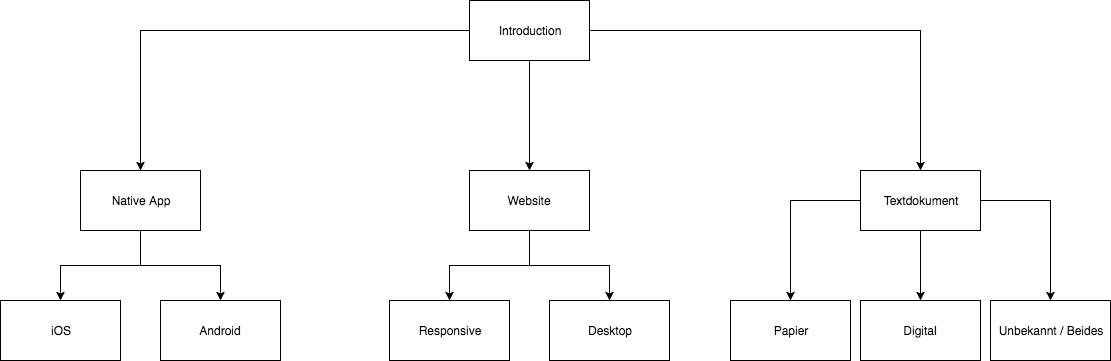
\includegraphics[width=1\textwidth]{images/ablauf_intro.png}
    \caption{Zielmedien der Nutzer und deren Unterkategorien}
    \label{fig:intro}
\end{figure}

Obwohl die Abgrenzung der Bereiche für die hier definierte Zielgruppe ausreichend ist, lassen sich bereits hier einige Stellen erkennen, die bei einer möglichen späteren Erweiterung der Zielgruppe überarbeitet werden müsste. Vorrangig betrifft das den Bereich \textit{Website}. Hier ist die vorhandene Unterteilung in \textit{Responsive} und \textit{Desktop} für ein Echtwelt-Szenario unter Umständen zu allgemein gehalten.

Hier gilt es außerdem festzulegen, wie genau der Nutzer der Anwendung sein jeweiliges Zielmedium mitteilen soll. Ziel muss es dabei sein, die kognitive Arbeit\footnotemark{} für diesen so gering wie möglich zu halten. Die in Abbildung \ref{fig:intro} gezeigte Struktur legt hier bereits eine Möglichkeit nahe, dem Nutzer immer nur eine Ebene des Baumes zur gleichen Zeit zu zeigen und so die Zahl der Auswahlmöglichkeiten so gering wie möglich zu halten.\\

\footnotetext{Als kognitive Arbeit werden Prozesse bezeichnet, die ein Nutzer durchführen muss, obwohl diese nicht sein eigentliches Anwendungsziel unterstützen. \cite[S. 410]{Cooper200903}}

Der Nutzer soll hierfür einen Wizard\footnotemark{} durchlaufen, der maximal drei Auswahlmöglichkeiten zur gleichen Zeit darstellt. Zur weitern Unterstützung und zur einfacheren Identifizierbarkeit der Optionen sollen die Interface-Elemente für die verschiedenen Auswahlmöglichkeiten außerdem aus Icon und Text bestehen.
Nach Beendigung des Wizards soll dem Nutzer seine getroffene Wahl noch einmal angezeigt werden, um so Fehler zu vermeiden, die unter Umständen zu einem späteren Zeitpunkt in der Anwendung den gesamten erarbeiteten Fortschritt nutzlos machen würden.

\footnotetext{``A \textbf{wizard} [...] is an enforced sequence of actions; [...]'' \cite[S. 418]{Cooper200903}}

\section{Typographie}
Durch die Umsetzung des Bereiches Typographie als Proof of Concept innerhalb des Praxisprojektes wurde hier bereits viel grundlegende Konzeptarbeit verrichtet, auf der hier aufgebaut werden kann.\\
Die Grundlegende Interaktion wurde dabei beibehalten: Weiterhin sieht der Nutzer einen Text, der sich auf seine Eingaben hin verändert. Die Eingabe erfolgt weiterhin primär über Slider, die in einer Tab-Navigation gruppiert sind. Die Platzierung dieser beiden Hauptelemente wurde jedoch verändert, sodass diese jetzt nebeneinander angeordnet sind, und nicht übereinander (vgl. Abbildung \ref{fig:vgl_poc_ba}). Diese Anordnung bietet die Möglichkeit, sowohl die Bedienelemente, als auch den gesetzten Text zu jeder Zeit sehen zu können und übermäßiges Scrollen zu vermeiden.\\
Eine weitere Verbesserung wurde im Bereich der Fehleranzeige vorgenommen: Hier wird über ein Icon in der Tab-Navigation deutlich gemacht, dass in einem bestimmten Bereich ein Fehler vorliegt.

\begin{figure}[h]
    \centering
    \includegraphics[width=1\textwidth]{images/vergleich_PoC_BA.png}
    \caption{Der Bereich Typographie, im Praxisprojekt und der Abschlussarbeit}
    \label{fig:vgl_poc_ba}
\end{figure}

Einen weiteren Ansatz stellt die direkte Interaktion mit Elementen dar. So bestünde beispielsweise die Möglichkeit, eine Überschrift anzuklicken und deren Attribute daraufhin direkt zu editieren. Hier wird, im Vergleich zur Interaktion mit Tab-Navigation und Schiebereglern, zwar schneller deutlich, auf welches Element die getätigte Eingabe wirkt, jedoch bietet dieser Ansatz auch einige Nachteile. So können sich Elemente innerhalb des Textes überschneiden (beispielsweise die gesamte Breite des Textes und ein einzelner Textabsatz), wodurch eine genaue Auswahl erschwert wird. Weiterhin ergeben sich Probleme bei einer übersichtlichen Fehleranzeige: Es stellt sich als kompliziert dar, deutlich zu machen, zu welchem Teil des gesetzten Textes ein Fehler zugehörig ist.\\
Da diese Art der Interaktion außerdem nicht sehr verbreitet ist und eine Erklärung für den Nutzer erfordern würde, wurde dieser Ansatz nicht weiter verfolgt.\\

Eine konzeptuelle Neuerung stellt ein Button zum zurücksetzen der Werte auf die Standardeinstellungen dar. In Situationen, in denen der Nutzer in verschiedenen Bereiche Werte verändert hat und mit diesen unzufrieden ist, bietet der Button eine komfortable Methode für einen Neustart des Schrittes.\\
Im Bezug auf die Standardeinstellungen stellt sich die Frage, welche Einstellungen hier zu verwenden sind. Es wurde sich bewusst gegen eine fehlerfreie Standardeinstellung entschieden, da es dem Nutzer nicht möglich ist, in der Anwendung einen Schritt vorwärts zu gehen, wenn noch Warnungen angezeigt werden. So kann sicher gestellt werden, dass der Nutzer sich auf jeden Fall mit dem Bereich Typographie befasst.
Auf der anderen Seite sollten die Standardeinstellung nicht zu viele Fehler enthalten, um den Nutzer nicht zu demotivieren. Hier wurde nur ein einziger Fehlerhafter Wert gewählt, der im ersten Tab zu sehen und dadurch mit wenig Aufwand zu beheben ist.\\

\section{Farben}
Während des Praxisprojektes wurde auch hier bereits ein grundlegendes Konzept aufgestellt. Die wichtigsten Punkte, in wenigen Sätzen zusammen gefasst, sind dabei:
Die Farbfindung geschieht in zwei Schritten, das finden der Grundfarbe und das Finden der Akzentfarbe. Farben sollen dabei auch nach Emotionen oder Adjektiven wählbar sein. Für die Betriebssysteme iOS und Android bestehen dabei gesonderte Regeln. \cite{PoplawskiPP}

Im ersten Schritt wurden die verschiedenen Darstellungen für die unterschiedlichen \textit{scopes} festgelegt.

\begin{itemize}
  \item \textbf{Finden einer Grundfarbe:} Hier wurde das Konzept aus dem Praxisprojekt übernommen. Für jeden \textit{scope} werden die jeweiligen Farben zu Auswahl gezeigt, wobei diese Auswahl bei den Mobilen Betriebssystemen durch deren Richtlinien begrenzt ist und somit in Form von Buttons realisiert werden kann.
Für die \textit{scopes} Website und Textdokument ist die Auswahl nicht begrenzt und die Selektion der Farbe findet hier durch einen Colorpicker statt.\\
Für den \textit{scope} Android werden bei einer Auswahl durch den Nutzer die Abstufungen 300 und 500 automatisch zum Farbschema hinzugefügt, um den Raum für Fehler so gering wie möglich zu halten.
  \item \textbf{Finden einer Akzentfarbe:} Für den \textit{scope} iOS entfällt dieser Schritt, für die beiden anderen Schritte wurde dem Nutzer die Möglichkeit gegeben, über Buttons die Art der Akzentfarbe zu wechseln (im Bereich Android über die Helligkeit, in anderen Bereichen in Form des gewählten Kontrastes).
  \item \textbf{Anzeigen des Farbschemas:} Wie bereits beim Einstieg in die Anwendung soll dem Nutzer am Ende das gesamte Farbschema angezeigt werden, bevor er zum nächsten Schritt in der Anwendung wechselt. Dies ist vor allem Nötig, weil der Nutzer während der Erstellung immer nur Teile des gesamten Farbschemas sieht.
\end{itemize}

Als schwierig gestaltete sich die Zuordnung von Farben zu bestimmten Adjektiven. Viele Quellen machen zwar angaben über die Wirkung von bestimmten Grundfarben, genaue Farbabstufungen (zum Beispiel in Form von HEX- oder RGB-Werten) lassen sich aber nicht finden. Ziel der Anwendung soll es aber sein, dem Nutzer einen Konkreten Farbwert zu empfehlen, mit dem dieser Arbeiten kann. \\
Die Farbfindung über Adjektive hat in der Anwendung vor allem den Zweck, dem Nutzer das Finden einer Farbe zugänglicher zu machen. Es ist \textbf{nicht} das Ziel der Anwendung, dem Artefakt des Nutzers eine bestimmte emotionale Wirkung zu geben. Daher ist hier ein subjektives Festlegen der genauen Farbwerte eine akzeptable Lösung. Konkret wurden aus \cite{Wright2017Color} und \cite{Cooper200903} verschiedene Adjektive zu den Grundfarben extrahiert, denen dann konkrete Werte zugewiesen wurden.

Dem Nutzer soll weiterhin, bereits während der Auswahl, eine möglichst genaue Vorstellung von der Wirkung der von ihm gewählten Farbe gegeben werden. Deswegen verfärbt sich ein großer Teil des Hintergrundes während dieses Schrittes entsprechend der Auswahl des Nutzers. Diese Hintergrundfärbung wird auch bei der Wahl der Akzentfarben beibehalten, wobei die Akzentfarben als kleinere Flächen auf der Grundfarbe angezeigt werden. Auch hier soll ein direkter Einblick in die mögliche spätere Verwendung geschaffen werden. Abbildung \ref{fig:colors_bg} zeigt diesen Ansatz im fertigen Produkt.

\begin{figure}[h]
    \centering
    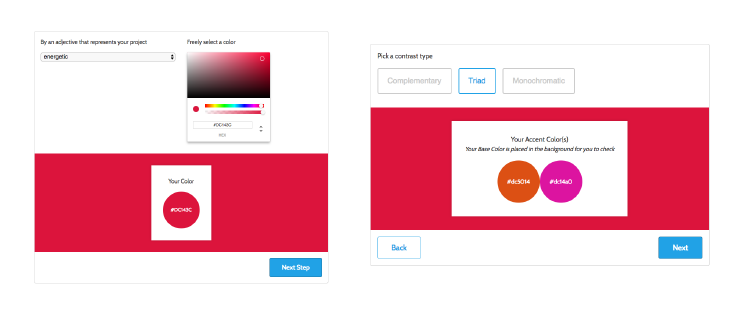
\includegraphics[width=1\textwidth]{images/colors_background.png}
    \caption{Vorschau der ausgewählten Farben in der Anwendung}
    \label{fig:colors_bg}
\end{figure}

\section{Layout \& Grid}

Im Bereich Layout und Grid zeigten sich die deutlichsten Unterschiede in der Art und Weise, in der die Anwendung auf das Entwicklungsziel des Nutzer reagiert.
So können für native Anwendungen im mobilen Bereich lediglich Empfehlungen und Verweise auf externe Quellen gegeben werden, während für Textdokumente die Möglichkeit besteht, währen der Anwendung konkrete Ergebnisse zu erarbeiten \cite{PoplawskiPP}.

Während der Arbeit wurde für die Bearbeitung von Textdokumenten das Layout an den Bereich Typographie angepasst, da die Interaktionen hier ähnlich sind und somit für den Nutzer eine einheitlichere Nutzungserfahrung geschaffen werden konnte.\\
Für den Bereich Web wurde eine Möglichkeit entworfen, bei der der Nutzer Erfahrungen mit der Arbeit von Grids sammeln kann. Hier wird dem Nutzer eine Seite mit abstrakten geometrischen Elementen dargestellt, über denen ein Grid liegt. Der Nutzer kann die Werte dieses Grids in drei Bereichen verändern: Anzahl der Spalten, breite der Spalten und Abstand zwischen den Spalten. Die dargestellte Seite verändert sich zusammen mit dem Grid und zeigt dem Nutzer so, welche Auswirkung eine Veränderung des Grids haben kann.

\subsection{Anmerkung zur Umsetzung}
Da dieser Bereich der bisher komplexeste ist, konnte eine Umsetzung im Zeitrahmen nicht realisiert werden, hier konnte nur die Arbeit im Bereich Konzept und Gestaltung finalisiert werden.
 Vor dem Gesichtspunkt, dass es Ziel der Arbeit ist, eine Marktfähige Anwendung in form eines MVP zu erstellen, wurde sich gegen eine Implementation dieses Bereiches in einem unfertigen Zustand entscheiden.\\
Die begonnene Arbeit in der Entwicklung an diesem Bereich wurde aber in Form eines \textit{Pull Requests} auf der Plattform Github veröffentlicht. Dieser soll Zeigen, dass die Anwendung auch in Zukunft weiter entwickelt werden soll und auch als Motivation für die aktive Mitarbeit von Dritten dienen.

\section{Ergebnisse der Benutzung}
\label{chap:results}
Auch wenn es eines der Hauptziele der Anwendung ist, dem Nutzer während seiner Nutzung interaktiv Wissen zu vermitteln, ist die Anwendung dennoch darauf ausgelegt, den Nutzer bei der Gestaltung eines konkreten Artefaktes zu unterstützen. Hier ist es für den Nutzer hilfreich, auf die von ihm erarbeiteten Ergebnisse auch nach der Verwendung des Tools noch Zugriff zu haben.

Dieser Bereich wurde im Rahmen des Praxisprojektes nicht konzipiert, ist aber für die Wahrnehmung der Anwendung als fertiges Produkt durchaus wichtig. Eine gute Darstellung der Ergebnisse des Nutzers definiert einen ausschlaggebenden Teil der Nutzungserfahrung, da ohne diesen Schritt das Gefühl aufkommen würde, dass während der Zeit der Nutzung kein Mehrwert erwirtschaftet wurde.
Im folgenden sollen also mögliche Darstellungen der Ergebnisse diskutiert und vorrangig die Frage beantwortet werden, welche Darstellungsweise den besten Kompromiss aus Umsetzbarkeit und Mehrwert für den Nutzer bietet.

Die einfachste Darstellung, die in jedem Falle gewählt werden sollte, ist eine transistente Darstellung am Ende einer Nutzung der Anwendung. Hier sollte dem Nutzer noch einmal aufgezeigt werden, welche Werte er innerhalb der Anwendung erarbeitet hat. Transistent ist diese Darstellung, weil diese zunächst nur im JavaScript-Programm im Browser des Nutzers gespeichert wird. Schließt dieser das Browserfenster, so wird auch das JavaScript-Programm beendet und die Ergebnisse gehen verloren.

Ein naheliegender Schritt ist also die Persistierung des Wissens für den Nutzer. Hierfür bieten sich verschiedene Möglichkeiten. \\
Denkbar wäre zum Beispiel das Speichern der Daten als Cookie\footnotemark{} im Browser des Nutzers. So könnten die Daten beim nächsten Besuch der Anwendung wieder angezeigt werden.
\footnotetext{Ein Cookie erlaubt das Speichern eines Zustandes über das HTTP-Protokoll \cite{rfc6265}}
Von Nachteil ist hier, dass die Kontrolle über die Speicherung der Daten nicht explizit beim Nutzer liegt: Löscht der Browser den Cookie (zum Beispiel, weil dessen \textit{Max-Age}\footnotemark{} Wert überschritten ist) sind die Daten ohne Eingriffsmöglichkeit des Nutzers verloren.\\
Eine andere Möglichkeit Bietet das Entwicklen eine Backends, das eine entsprechende Datenhaltung verwalten kann. Hier könnten auch mehrere Projekte eines Nutzer gespeichert werden, allerdings liegt der Entwicklungsaufwand für ein solche Backend außerhalb des zeitlichen Rahmens der Abschlussarbeit. \\
Als Kompromiss zwischen Nutzerfreundlichkeit und Entwicklungsaufwand wurde sich für die Persistierung des Wissen in einer Datei im PDF-Format entschieden, die der Nutzer Herunterladen kann.

\footnotetext{Das \textit{Max-Age} Attribut kennzeichnet die maximale Dauer, die ein Cookie im Browser behalten wird. \cite{rfc6265}}

Weitere Verbesserungen der Nutzererfahrung können im Aufbau und Inhalt der Datei erreicht werden. Optimal wäre eine Aufbereitung der Daten, sodass der Nutzer diese möglichst ohne weitere Bearbeitung in seinen Workflow übernehmen kann. Obwohl das Zielmedium des Nutzers bekannt ist, können daraus keine zweifelsfreien Rückschlüsse auf die benötigte Struktur und Form der Daten gezogen werden. \\
So kann beispielsweise bekannt sein, dass der Nutzer eine Webanwendung entwickelt und das Setzen seiner Texte in der CSS-Syntax vornimmt. Trotzdem kann der Nutzer zum Beispiel verschiedene Preprozessoren wie SCSS, SASS oder LESS verwenden, die jeweils eine unterschiedliche Syntax verwenden.
Oder es kann bekannt sein, dass der Nutzer an einer Textseite arbeitet, jedoch nicht, welches Textsatzprogramm er verwendet\footnotemark{}.\\
\footnotetext{Ein weiteres Problem stellt die Aufbereitung der Daten für einen Import in ein Textsatzprogramm dar.}
Es ist dabei durchaus Möglich, die benötigten Informationen vom Nutzer zu erhalten und die Daten in Einzelfällen entsprechend aufzubereiten, jedoch liegen auch diese Anforderungen außerhalb des Zeitlichen Rahmens dieser Abschlussarbeit.
